\begin{definition} \textbf{Conjunto simplemente conexo en el plano.} \label{def:conjuntosimpleconexo}
   Sea $A \subseteq \mathbb{R}^{2}$ un conjunto conexo. Decimos que $A$ es \emph{simplemente conexo} si para toda curva continua, simple y cerrada contenida en $A$, la región interior que dicha curva encierra está completamente contenida en $A$.
\end{definition}

\begin{center}
        \begin{minipage}{0.45\textwidth}
            \centering
            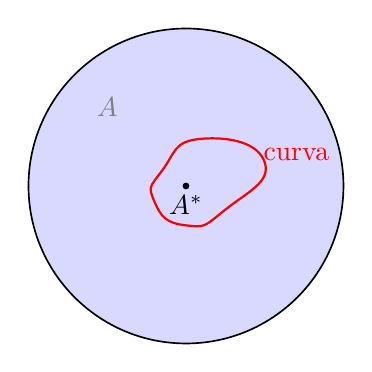
\begin{tikzpicture}
                \draw[fill=blue!15, semithick] (0,0) circle(2);
                \draw[red, thick]
                plot [smooth cycle, tension=1] coordinates {
                    (-0.3,0.2)
                    (0.2,0.6)
                    (1,0.3)
                    (0.5,-0.3)
                    (0,-0.5)
                    (-0.4,-0.2)
                };
    
                \node at (-1,1) {\textcolor{gray}{$A$}};
                \node at (1.4,0.4) {\textcolor{red}{curva}};
                \filldraw[black]  (0,0) circle (1pt) node[below]  {\( A^{*} \) };
            \end{tikzpicture}
        \end{minipage}
    \hspace{1cm}
        \begin{minipage}{0.45\textwidth}
            \centering
            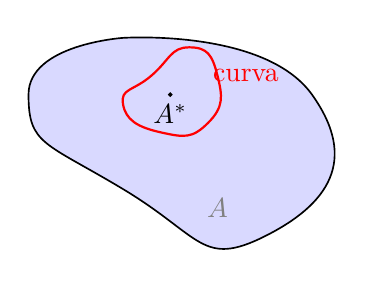
\begin{tikzpicture}[scale=1.2]
                \filldraw[fill=blue!15, semithick]
                    plot[smooth, tension=1.2] coordinates {(1,0.6) (3,0) (2.5,-1.5) (1,-1) (0,0) (1,0.6)};
                    \draw[thick, red]
                    plot [smooth cycle, tension=1] coordinates {
                        (1.3,0.2)
                        (1.7,0.5)
                        (2,0.2)
                        (1.9,-0.3)
                        (1.4,-0.4)
                        (1,-0.1)
                    };
                \node at (2,-1.2) {\textcolor{gray}{$A$}};
                \node[red] at (2.3,0.2) {curva};
                \filldraw[black] (1.5,0) circle (0.5pt) node[below] {\( A^{*} \) };
            \end{tikzpicture}
        \end{minipage}
    \end{center}
    
    \vspace{0.3cm} % Pequeño espacio antes de la etiqueta
    
    \begin{center}
        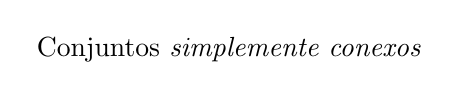
\begin{tikzpicture}
            \node at (1.5,-2) {Conjuntos \emph{simplemente conexos}};
        \end{tikzpicture}
    \end{center}
    
  %  \begin{center}
    %    \begin{tikzpicture}
            % Círculo exterior (azul claro) \draw[fill=blue!15, semithick] (0,0) circle(2);
    %        \draw[fill=blue!15, semithick] (0,0) circle(2);
            
            % Círculo interior (blanco, para el hueco)
  %          \draw[fill=white, semithick] (0,0) circle(0.8);
   %         \draw[red, thick]
     %       plot [smooth cycle, tension=1] coordinates {
      %          (0.7,0.1)
     %           (1,0.5)
     %           (1.4,0.2)
      %          (1.3,-0.3)
     %           (0.9,-0.5)
      %          (0.6,-0.4)
       %         (0.5,-0.1)
        %    };
       %         \node at (-1,1) {\textcolor{gray}{$A$}};
      %          \node at (1,0.9) {\textcolor{red}{curva}};
      %          \filldraw[black] (1,0) circle (0.5pt) node[below] {\( A^{*} \) };;
      %  \end{tikzpicture}
      %  \end{center}
      %  \begin{center}
       %     \begin{tikzpicture}
        %        \node at (1.5,-2) {Conjunto \emph{no simplemente conexo}};
        %    \end{tikzpicture}
       % \end{center}       
  

\begin{definition} \textbf{Conjunto simplemente conexo en $\mathbb{R}^{n}$.} \label{def:conjuntosimpleconexo2}
Sea $A \subseteq \mathbb{R}^{n}$ un conjunto arcoconexo.  Decimos que $A$ es \emph{simplemente conexo} si toda curva continua y cerrada contenida en $A$ puede deformarse continuamente dentro de $A$, manteniendo su punto inicial y final fijos, hasta reducirse a un único punto.
\end{definition}




\includegraphics{tikz/standalone_fig_lazo.pdf}

    
    
    
       
    
    
    
    
    
    
    